% !TeX root = RJwrapper.tex
\title{Analyzing Dependence between Point Processes in Time Using \pkg{IndTestPP}}
\author{by Ana C. Cebrián and Jesús Asín}

\maketitle

\abstract{The need to analyze the dependence between two or more point processes in time appears in many modeling problems  related to the occurrence of events,  such as the occurrence of  climate events at different spatial locations or  synchrony detection in spike train analysis. The package \pkg{IndTestPP}  provides a general framework for  all the steps  in this type of analysis, and one of  its main features is the implementation of three families of tests to study  independence given the intensities of the processes, which are not only useful to assess independence but also to identify factors causing dependence. The package  also includes functions   for  generating different types of  dependent point processes, and implements computational statistical inference tools using them.   An application to  characterize the dependence   between the occurrence of extreme heat events in  three Spanish locations   using the package is shown.
}

	\section{Introduction}
%% Note: If there is markup in \(sub)section, then it has to be escape as above.


A point process  in time (PP in short) is a random collection of points  in a space in $\mathbb{R}^+$  where each point  usually represents the time of an event.  Examples of  events that can be
modeled as point processes in time include the occurrence of earthquakes, heat waves, or  the arrivals of insurance claims.
Many  real problems  involve not one but two or more   PPs, and they should be studied in a multivariate  framework where a  description  of the independence or dependence structure between them is required.   Examples of these situations are the timing of the trades and mid-quote changes  in the stock exchange,  the occurrence of temperature extremes or other climate events at different spatial locations, or  the synchrony detection in spike train analysis.

In those situations, statistical tests are required to assess the independence between two or more PPs.  If we can assume  that the  processes are independent, their modeling is much simpler, since it can be carried out separately for each process without any loss of information.  The  tests are also useful  to identify the type of dependence and  select  the type of vector of point processes  used to model them.    The need  of  testing independence  between PPs appears in   climate and environmental sciences   \citep{Cronie16, Abaurrea15}, in  neuroscience  \citep{Tuleau14, Albert15}, in  biology \citep{Myllymaki17},  and many other fields.


Two types of independence between PPs  may be of interest,  general independence \citep{Rubin14} and  independence,  given the intensities of the  processes. The election  of the type of independence  as null hypothesis  depends on the aim of the study, but  the second type  is more  useful in  modeling problems based on PPs.  In effect,  the most frequent approach to model  systematic dependence structures caused by common factors  is
the use of nonhomogeneous processes with intensities, which are  functions of   the same or dependent covariates.  To analyze if the dependence is well  represented by those covariates,  the  null hypothesis of independence given the intensities  has to be checked.
When  the existing dependence cannot be explained by the available covariates,   models taking into account that dependence should be considered to model the vectors of PPs.

The R package \CRANpkg{IndTestPP} \citep{IndTestPP} provides a general framework for  all the steps to analyze the dependence in a vector of point processes in time:  from data  processing and tests of independence to   inference  tools for parameters of interest.   That makes it a useful tool for applications based on the modeling of a vector of point processes. As far as we know, there is  not other software for this type  of analysis. One of the main features  of the package is the implementation of the three families of independence tests by \citet{Cebrian20}, which  cover a wide variety of homogeneous and nonhomogeneous processes appearing in real problems:  Poisson processes, processes with a  parametric marginal model,  point  processes with  known marginal intensities,  etc.  The package also provides functions to generate  four different models of dependent PPs, and two types of independent PPs,  which are  useful to develop inference tools based on computational statistical  methods. 



The outline of the paper is as follows.  The two first sections \textit{Vector of point processes in time} and \textit{Point processes in R} introduce  some properties for vectors of point  processes and some R packages related to this topic.
The three following sections describe the   implementation in R of  the  tests of independence, the measures of dependence, and the tools for generating PPs.  The final section  shows  an  illustrative example of an analysis to  characterize the dependence   between the occurrence of extreme heat events in  three Spanish locations using  \pkg{IndTestPP}. 



\section{Vectors of point processes in time} 

\label{VectorPP}

A point process in time, $N$, is defined  in $\mathbb{R}^+$ and  can be described  in  different   equivalent ways. Here, we will mainly use  the sequence of  occurrence times, $T_1, T_2, ..., T_n$,  and also  the set of random variables $N(A)$ representing the number of points in $A$, for each $A \in  \mathbb{R}^+$.  The notation for $A=(0, t]$  is $N(t)=N((0,t])$.  
The intensity measure of the process $\Lambda$ gives the expected number of points in  a set,  so that $\Lambda((0,t])=E(N((0,t]))$.
Its derivative function, provided it exists, is  the intensity function,
$$
\lambda\left(t\right)=\frac{\partial \Lambda\left(\left(0, t\right]\right)}{\partial t}.
$$



If the intensity is constant,  the process is homogeneous and  nonhomogeneous  otherwise. The most known PP is the Poisson process,  where  $N(A)$  has a $Poisson(\mu_A)$ distribution, with $\mu_A=\int_A \lambda(t) dt$, and $N(A_1), \ldots N(A_k)$ are independent variables provided that $A_i \cap A_j= \emptyset ,\ \  \forall i \ne j$.


Herein,   we will consider vectors of point processes  $\mathbf{N}=(N_1, \ldots, N_d)$	observed in  the same  space $\Omega=(0, T] \subset \mathbb{R}^+$. This definition  must not be  mixed up with	a multivariate point processes  defined as a process of random points $\mathbf{X_i}=(X_{i1},\ldots, X_{id})$   in a d-dimensional space $V\in \mathbb{R}^d$,
whose simplest example with $d=2$ is a spatial point  processes.  Figure \ref{Fig1a}  shows  the differences between the two concepts with $d=3$. 
 A vector of PPs can be seen as a  marked point process with discrete marks, and   can be represented by a countable collection of pairs  $(T_i, D_i)$ where  $T_i \in \mathbb{R}^+$ are the  occurrence times and $D_i \in \{1, \ldots , d\}$ are the component indexes.


Most of the results  in this work are developed  for  vectors of $d=2$ processes,  denoted by $(N_x, N_y)$ with intensities $\lambda_x(t)$ and $\lambda_y(t)$. If the results  can be extended to  higher values of $d$, it is specified. The  $n_x$ and $n_y$  points in  each observed  process are denoted	$t_{1}, \ldots, t_{n_x}$ and  $s_{1}, \ldots, s_{n_y}$,  respectively.



\begin{figure}[t]
	\begin{center}
		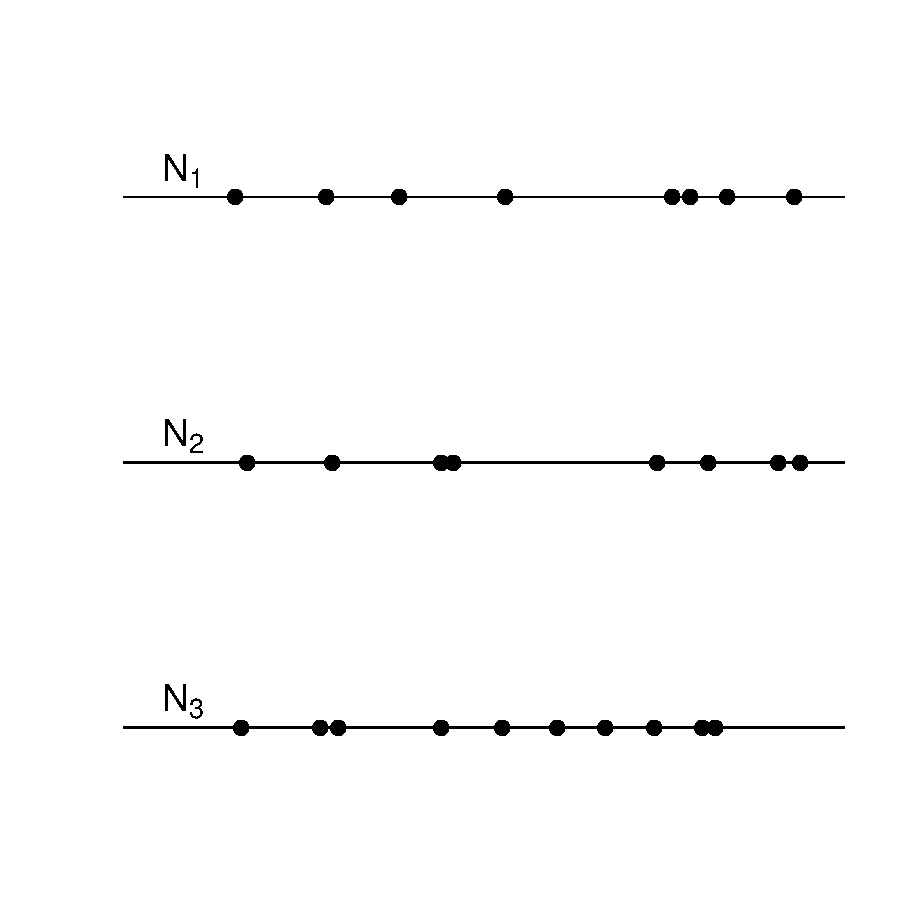
\includegraphics[width=0.4\textwidth]{figure/graficod3.pdf}
		\hspace*{1cm}
		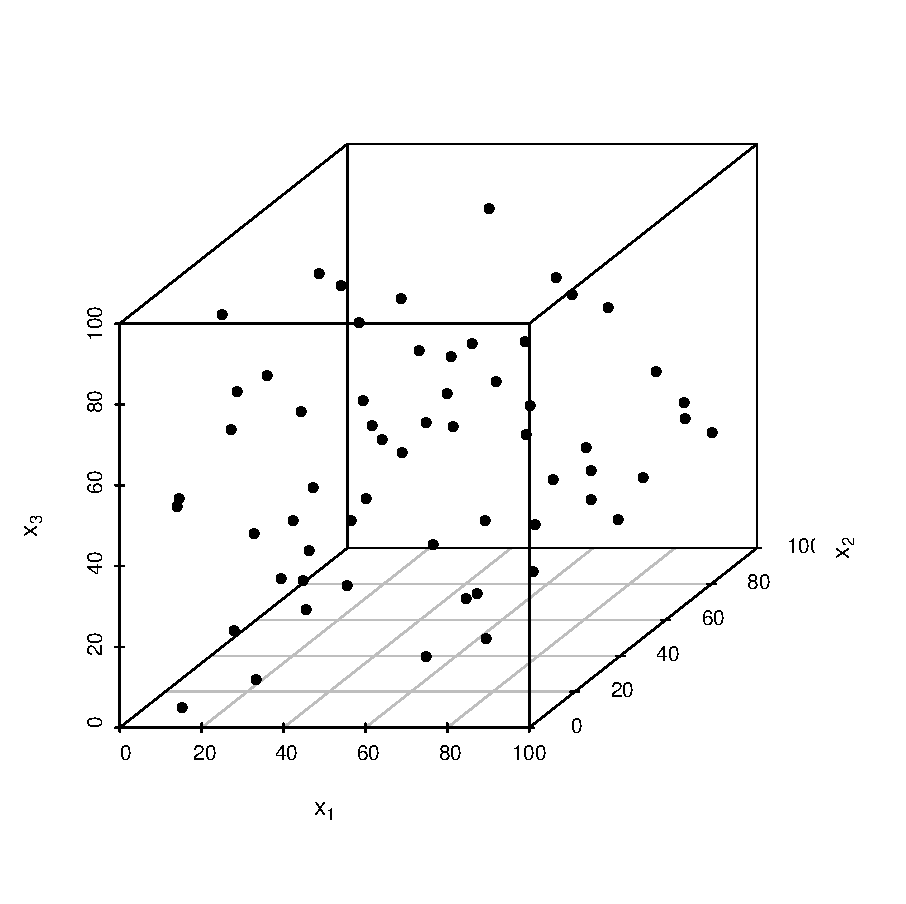
\includegraphics[width=0.48\textwidth]{figure/grafico3d.pdf}
	\end{center}
	\caption{\label{Fig1a} Vector of    three point processes (left), and  multivariate point process  in a tridimensional space (right).}
\end{figure}



Many  types of dependence structures  can appear  between  the marginal processes of a vector. The most direct way of modeling it is to use   models   to represent  the dependence between the occurrence times  of the  processes, such as the common Poisson shock processes,  the queue processes, the Poisson processes  with dependent marks, or the  multivariate Neyman-Scott processes, described later.





\section{Point processes in R}


\label{Section3}


There exist many  packages  in R devoted to the analysis of spatial  point processes: the extensive  \CRANpkg{spatstat} \citep{Baddeley15},  whose main  functionalities include exploratory data analysis, model-fitting, and simulation,   \CRANpkg{stpp} \citep{stpp}, \CRANpkg{splancs} \citep{splancs}, and many others. \CRANpkg{IDSpatialStats} \citep{Giles19} provides spatial dependence measures, and future directions include  the  extension to the  spatio-temporal case. However, the  number of packages  dealing with the analysis of point processes in time  is not so high, and most of them deal with  univariate analysis of the processes.  \CRANpkg{NHPoisson} \citep{Cebrian15}   provides a global framework for the  modeling and diagnosis of  Poisson processes in time,  \CRANpkg{PtProcess} \citep{PtProcess} fits and analyses time-dependent marked point processes with an emphasis on earthquake modeling, and \CRANpkg{mmpp} \citep{mmpp} offers various similarity and distance metrics for marked point processes.

 
 
The aim of \pkg{IndTestPP}  is the analysis of vectors of point processes in time, in particular of its dependence, and it  provides a general framework  for  all the steps involved in  this type of analysis:   data processing,  estimation of the marginal intensities of the processes,   analysis of  independence given the intensity, identification of factors causing  dependence, and inference  tools  based on computational statistics. 
\CRANpkg{mppa}  \citep{mppa} provides a test for dependence between point processes on the real line, but   with a different aim since it tests general independence. The three families of tests implemented in \pkg{IndTestPP}   are more general since they are not restricted to Poisson processes, and they  test independence given the  marginal intensities. This type  of  conditional independence is more useful in  statistical modeling of vectors of point processes since it helps to identify the factors  that cause the dependence. An example of how all the steps of the modeling  of  a vector of point processes can be carried out using \pkg{IndTestPP} is shown in  the application section.

 


\section{Testing independence between point processes in time}

\label{Section4}

 Most of the analysis of independence  between point processes in the literature  involve  spatial processes, but few works deal with the study of independence between processes in time. \pkg{IndTestPP} includes the  three families of tests   to assess independence between PPs in time by \citet{Cebrian20}, i.e.,  the POISSON, the CLOSE, and  the CROSS families, and a graphical tool, the Dutilleul plot. In all of  them, the null hypothesis  is the  independence between the point processes, given their  marginal intensities, and the alternative the existence of any type of random dependence between them. All the tests  in these families  are constructed by keeping fixed  the first  observed  process,  a common approach to test independence given the marginal structure. However, each test is based on different assumptions, and  all together they  cover a wide range of types of processes appearing in real problems.



\subsection{POISSON family}


The  family of tests POISSON is implemented in  the  function \code{CondTest},  and it includes two  tests to assess the independence between  two homogeneous or nonhomogeneous processes,  based on the  conditional distribution of  $N_y |N_x$.  The  assumptions of the tests are  that  $N_y$  is a Poisson process with intensity function  $\lambda_y(t)$, specified in  the vector argument \code{lambday}.

This family is  based on the following  property.  If $N_x$ and $N_y$  are independent, and  a point $t_i$ occurs in  $N_x$,    the distribution of  $N_y$  does not change. Then,   $Y_i$, the number  of points   in $N_y$ in  intervals $l_i$ of length $2r$ around $t_i$, follows  a $ Poisson(\mu_i)$ distribution with $\mu_i=\int_{l_i} \lambda_y(t) dt$.

Two  options are available to  perform a test. The test implemented with the argument \code{type='Poisson'}  is based on  the fact that under the  independence between $N_x$ and $N_y$ and if not overlapping intervals  are used, the  statistic  $Y=\sum_{i=1}^{n_x} Y_i$ has a $Poisson(\mu)$ distribution  with $\mu=\sum_{i=1}^{n_x} \mu_i$. 
A  test based on a Normal approximation  is  implemented with the  argument \code{type='Normal'}.    Again, under the null  and with not overlapping intervals, the variables $(Y_i-\mu_i)/\sqrt{\mu_i}$ are     zero mean   independent variables with standard deviation equal to 1, and  the asymptotic distribution  of the statistic
$$O_{n_x}=  {1 \over \sqrt{n_x}}\sum_{j=1}^{n_x}{Y_j-\mu_j\over \sqrt{\mu_j}}$$
is  $N(0,1)$.	If  the  argument  is \code{type='All'}, both tests are calculated. 

The intervals  where the number of points is counted, $l_i$ , are centered intervals around  points $t_i$ of radius $r$ specified  by the  argument \code{r}. If 
 \code{changer=TRUE},  when two  intervals overlap, their lengths are  shortened by half of the intersection period; in this way  the  resulting intervals are disjoint and, consequently,  the corresponding variables $Y_i$  are independent.

The power study  by \citet{Cebrian20} shows that the  Normal test  performs better provided that conditions to guarantee the normal approximation are fulfilled.  These conditions are quite weak,  even  with  a complex intensity,  mean values  of $\mu_i$ around 0.6  points per interval lead to a valid approximation with $n_x=50$, and around  0.3 with $n_x=100$.



\subsection{CLOSE family}
\label{CLOSEtests}


The CLOSE family includes two tests,  the parametric bootstrap (PaB) and the Lotwick-Silverman (LoS) tests,  implemented in the  functions  \code{TestIndNH} and \code{TestIndLS}, respectively. The  LoS test can only  be applied  to  homogeneous processes, but  the PaB  test also to  nonhomogeneous ones. On the other hand, the LoS does not require any assumption to be applied, while PaB requires that $N_y$ follows a parametric model  with a generation algorithm, such as a Poisson or a Neyman-Scott cluster process.	
Although both tests allow  checking the independence between $d$ processes in general, the  calculation of the statistic is only implemented for $d=2$ and $d=3$.


These tests  are based on the  close point  distance, and they aim to compare the behavior  of the  sets of close points in a vector of observed  processes and in  vectors with the  same  marginal distributions but  independent components \citep{Abaurrea15}.
A point $s_j$  in $N_y$ is a close point of $t_i$ in $N_x$ if the intervals to their previous points, $s_{j-1}$ and $t_{i-1}$, overlap. The set behavior is summarized by $\bar dx_i$, the mean of  the distances between $t_i$ and  its close points, $|s_j-t_i|$.  The set of close points and the mean distance for each point $t_i$ are calculated by the functions \code{uniogentri} and \code{DistObs}, respectively.  


Given the complexity of the test statistic, its distribution  has to be obtained by computational statistical methods. These methods  require approaches  to generate a sample of $r$ processes $N^*_j=(N_{x}, N^*_{y,j})$, where  the observed process $N_x$  is fixed,   $N^*_{y,j}$   has the same  distribution as $N_y$,  and $N_x$ and $N^*_{y,j}$ are independent. The PaB and LoS tests result from two  different generation approaches.


\textbf{Parametric bootstrap test}.  In this test, the  $N_{y,j}^*$ processes  are generated  independently from   $N_x$  using   a parametric model. Two types of marginal  models are implemented in \pkg{TestIndNH}: Poisson processes (\code{type="Poisson"})   and   Neyman-Scott cluster processes  (\code{type="PoissonCluster"}).The generation of Poisson processes  in a given period uses the function \code{simNHPc}, based on a two-step algorithm which   generates homogeneous occurrence times, and transform them into 
the points  of a  NH process with intensity $\lambda(t)$ \citep{Ross06}.
Neyman-Scott cluster processes  are obtained by the function \code{IndNHNeyScot}. Details about these processes  are explained later.


\textbf{Lotwick-Silverman test (LoS)}.   \code{TestIndLS} generates  processes    using   a Monte Carlo method conditional on the observed marginal structure \citep{Lotwick82}. 
The  steps   are the following:
\begin{itemize}
	
	\item[1.]  The  observed  processes $(N_x, N_y)$ are wrapped onto a circumference by identifying the  opposite sides of the time interval where they are observed.
	\item[2.] Fixing $N_x$, a new $N^*_y$ is generated by translating $N_y$  a random   uniform amount  on the circumference. This breaks any dependence between the processes and  keeps the marginal distributions, provided they do not change over time.
\end{itemize}



The mean distances  of the close point sets in  the generated vectors of processes in the PaB and the LoS tests  are calculated by the functions  \code{DistSim} and \code{DistShift},  respectively.
The  calculation of the \emph{p}-value requires the generation of processes in two steps of the algorithm, to  calculate the   expectation of the mean   distances $\bar dx_{ij}$  and  to estimate  the distribution of the  statistic  in a correlated sample. This calculation is implemented  so that the  same  generated processes  are  used in the two steps and the computing time  is kept low; otherwise,  it would be multiplied by the number of  simulations. Moreover, parallel computation is implemented.


According to the power study by \citet{Cebrian20},  both LoS and PaB tests  have high power, but  LoS   performs slightly  better in the homogeneous processes with small samples and low dependence.





\subsection{CROSS family}

The CROSS family includes two tests based on  the cross K and the cross J spatial functions adapted to the case of PPs in time,  implemented in the  functions  \code{NHK} and \code{NHJ}, respectively.  These functions also  provide  estimators of the  cross functions. They do not require any assumption about the  distribution of the marginal processes, only to know their intensities, and the \emph{p}-values are calculated using a LoS approach. 	The tests can be applied to two homogeneous or  nonhomogeneous processes, and  more generally to two sets 
of processes, $\mathbf{C}=(N_{x1}, N_{x2}, \ldots, N_{xl_C})$ and $\mathbf{D}=(N_{y1}, N_{y2}, \ldots, N_{yl_D})$. 	
The information about the processes  is provided by  arguments \code{posC},  a vector containing all the occurrence times  in the processes in $\C$, and  \code{typeC},  a vector containing  the code $j$ of the process $N_{xj}$   where each point in \code{posC} occurs;  $\mathbf{D}$ is specified analogously by \code{posD} and \code{typeD}. For the sake of simplicity, the  results  are  expressed for the case,  $\mathbf{C}=(N_x)$  and $\mathbf{D}=(N_y)$  with intensities $\lambda_x(t)$ and $\lambda_y(t)$. 


\paragraph{K-function.}
 $K_{xy}(r)$ is the expected value of the number of points in $N_y$ within a distance $r$ of a randomly chosen point in $N_x$, adjusted for the possible time-varying intensity. 	
 \code{NHK} calculates two different estimators of  $K_{xy}(r)$  at a given grid of $r$ distances, and the corresponding test statistics based on them,  $\mathcal{K}=\frac{1}{R} \sum_{r=r_1}^{r_R}\hat K_{xy}(r)/2r$.    The estimator calculated by default  (\code{typeEst = 2}) performs better in terms of size and power  \citep{Cebrian20}.	


\paragraph{J-function.}

It compares the functions  $D_{xy}(r)$ (distribution function of the distances from a  point  in  $N_x$ to the nearest point in $N_y$) and  $F_{y}(r)$ (distribution function of the distances from a point   in the space to the nearest point in  $N_y$), in terms of the ratio $J_{xy}(r)=(1-D_{xy}(r))/(1-F_{y}(r))$,  if $F_{y}(r)<1$.  

The estimators of  $D_{xy}(r)$ and  $F_{y}(r)$, calculated by   \code{NHD} and  \code{NHF}, are  used  in   \code{NHJ} to estimate  $J_{xy}(r)$.  To estimate $F_{y}(r)$, a grid  of $L$ values is required. It can be provided in argument \code{L} or an automatic selection is calculated otherwise.	In the homogeneous PPs,  the  previous estimators  are equal to  the empirical  distribution functions,  and the  calculation algorithms are changed to reduce the computational cost. The test   statistic,  which  summarizes  the deviations  of the function from 1, is  
$\mathcal{J}=\frac{1}{R}\sum_{r=r_1}^{r_R}|\hat J_{xy}(r)-1|$.


In both functions, \code{NHK} and \code{NHJ}, the  grid of $r$ distances where the estimators are evaluated are  provided  in argument \code{r}. If it is NULL, an automatic  selection  based on length $T$  is carried out.
The  test statistics are also evaluated at  that grid, and since	dependence   often appears between close observations,  the  addends  with high $r$   can make it more difficult to discriminate  between dependent and independent processes. To avoid that effect,  the statistic can be calculated using only the addends with  $r<r0$  by using the argument \code{rTest=r0}. To identify an adequate value of $r0$,  values $\hat K_{xy}(r)$ or $\hat K_{xy}(r)/2r$   can be optionally  plotted.   




\paragraph{Computation of the \emph{p}-values.}   The calculation of the \emph{p}-value in  CROSS  tests is based on a LoS approach  for nonhomogenous processes.  First, the  observed  processes $(N_x, N_y)$ are wrapped onto a circumference. Then, fixing $N_x$, a new $N^*_y$ is generated by translating $N_y$ and  its  intensity $\lambda_y(t)$,  a random   uniform amount. This breaks any dependence,  but in nonhomogeneous PPs,  it   changes the distribution of the marginal processes. However, since    the  cross functions are adjusted  for the time-varying intensity,  which is also translated,  valid samples of  $K_{xy}(r)$ (or $J_{xy}(r)$)   under  independence  are obtained. 
Using the empirical distribution of those samples,  the \emph{p}-value  and
 confidence  envelopes for  $K_{xy}(r)$ (or $J_{xy}(r)$) are obtained.  Parallel computation is implemented  for these calculations.

\subsection{Dutilleul plot} 
 
 The function \code{DutilleulPlot} carries out  Diggle's randomization testing procedure extended by \citet{Dutilleul11}, which graphically assesses the independence between two homogeneous or nonhomogeneous Poisson processes, given their marginal structure.  The idea is to plot the cumulative relative frequency of the nearest neighbor distances between the points in the two observed processes and  to analyze the independence  using a confidence band  calculated from 	simulated  independent Poisson processes with the observed  marginal  intensities. 




\section{Dependence measures}

Unfortunately,  there does not exist a  general   definition to quantify the dependence between two PPs. However, we suggest some measures implemented in \pkg{IndtestPP} which can be  useful  to describe the  level of dependence between  many types of processes.

\label{Section5}

\textbf{Correlation between  the counting variables of two PPs}. 
  \code{CountingCor}  calculates  a sample estimator of   $\rho_{xy}^{L}=Cor(X_{i}, Y_{i})$, the correlation coefficient between  $X_{i}$ and $Y_{i}$ the  number of points in  processes $N_x$ and   $N_y$,  in an  interval $l_i$ of length $L$,  using a partition of the observed period. Given the discrete character of  $X_{i}$ and $Y_{i}$, and since the usual aim is  to quantify any type of dependence,  not only linear correlation,  Spearman  or Kendall  coefficients are   often more adequate.   Kendall should be preferred with  short intervals since there  will  be a high number of 0 or 1 occurrences per interval, and  the Kendall Tau-b  coefficient implemented in the function makes an adjustment for the ties. 


In nonhomogenous processes,   variables   $X_{i}$  (and $Y_{i}$)  in  intervals measured at different times are not i.d. In the case of Poisson processes,     \code{CountingCor}  can calculate a standardized  version of the  measure, so that all the variables   have the same mean and variance, and if  
$\Lambda_{x,i}= \sum_{t \in l_i}\lambda_x(t)$  and  
$\Lambda_{y,i}= \sum_{t \in l_i}\lambda_y(t)$ are high enough,  they  are also i.d.,
$$\rho_{xy}^L=Cor\left({X_{i}-\Lambda_{x,i} \over \sqrt{\Lambda_{x,i}}},   {Y_{i}-\Lambda _{y,i} \over \sqrt{\Lambda_{y,i}}}\right).
$$
This coefficient measures the correlation given the marginal intensities.  That means that the coefficient measures the correlation once that dependence captured by the intensities (through common covariates, for example) has been removed.



\textbf{Percentage of  concordant intervals.}	 A simpler descriptive measure   is the percentage of  concordant intervals, that is,  the percentage of intervals with occurrences in both processes. It is calculated by  \code{BinPer} as $n_{x,y}/(n_{x,y}+n_{x,0}+ n_{0,y})$, where $n_{x,y}$ is the number  of intervals with at least one point in both processes, and  $n_{0,y}$  and  $n_{x,0}$  are the number of intervals with at least one point in  one process and 0 in the other.  This percentage will tend to be zero in short intervals of independent processes, while  positive values  will suggest positive dependence. An adequate length of interval  that depends on the  marginal intensities has to be selected to obtain useful interpretations. 

\textbf{Extremal dependence coefficients.} In the case of  PPs resulting from a Peak over threshold (POT) approach, another interesting measure is the extremal dependence between the variables $X$ and $Y$ where the POT approach is applied. The extremal dependence is the tendency for one variable to be large, given that the other one is large. The  extremal dependence coefficient $\chi$  of $X$ given $Y$  is defined as $\chi_{x|y}= \lim_{u \to 1} \chi_{x|y}(u)$, where
$$\chi_{x|y}(u)= P\left(U>u |V>u\right),$$
and  $(U,V)$ are  the  transformed uniform marginals of  $X$ and $Y$. Another extremal
coefficient  is 
$\bar \chi_{x|y}= \lim_{u \to 1} \bar \chi_{x|y}(u)$, where 
$$\bar \chi_{x|y}(u)= 2 \ {\log P\left(U>u\right) \over \log P\left(U>u, V>u\right)}-1.$$


$\chi_{x|y}$ is on the scale $[0, 1]$, with the set $(0, 1]$ corresponding to asymptotic
dependence, and the measure $\bar \chi_{x|y}$ falls within the range $[-1, 1]$, with  $[-1, 1)$ corresponding to asymptotic independence. 
Thus,  ($\chi_{x|y} > 0$, $\bar \chi_{x|y} =1$) signifies asymptotic dependence,  and the value of $\chi$ determines  the strength of dependence within that class;  ($\chi_{x|y}=0$, $\bar \chi_{x|y} <1$) signifies asymptotic independence,  and $\bar \chi_{x|y}$  determines the strength of dependence within that class.
Full details can be found in \citet{Coles99}. 

The function \code{depchi} estimates the  functions  $\chi_{x|y}(u)$ and $ \bar \chi_{x|y}(u)$ in a given grid of values $u$. Both $\chi_{x|y}(u)$ and   $\chi_{y|x}(u)$  (or $\bar \chi_{x|y}(u)$ and   $\bar \chi_{y|x}(u)$) are calculated and optionally plotted. These graphs are useful to estimate the limit of the function and obtain $\hat \chi_{x|y}$ (and $\widehat{\bar \chi}_{x|y}$). In the plot of  $\chi_{x|y}(u)$, the expected behavior under independence  is also plotted.







\section{Generating point processes with different  dependence structures}

\label{Section6}

The generation  of vectors of  PPs with a given dependence structure is   necessary  to implement Monte Carlo,  parametric bootstrap,  or other inference methods based on simulation, such as those described in section  \textit{Inference based on computational statistical methods}. There are different approaches to model the dependence between the  marginal processes in a vector  of PPs, but  the most direct way is to   model  the dependence between the occurrence times  of the  processes.   \pkg{IndTestPP} includes  functions for the generation of four types  of vectors of homogeneous or nonhomogeneous PPs,  which will be described later in this section:  common Poisson shock processes,  multivariate Neyman-Scott processes, queue processes, and marked Poisson processes. 
These types of vectors allow  modeling  three dependence structures   frequently observed in real problems.   




\begin{itemize}
	
	
	\item[\textbullet] \textit{Dependence between two or more PPs provoked by  the same shock  triggering event}.  This  is   the most common dependence structure and can be modeled  by  a common Poisson shock process (CPSP) or  a multivariate Neyman-Scott process (MNSP).  Both models  show a short-term  and positive dependence, generated by  common shocks, but  in each one, the shocks  yield points in the processes  in a different way.	 This dependence appears in the spike trains of two neurons,  in climate and environmental processes,  or in financial problems,  for example,  when a political crisis provokes the occurrence of  large decreases in   different economical indexes.
	
	
	\item[\textbullet]  \textit{Dependence between shifted processes}. This is  a   point-to-point dependence, where the occurrence of an event in a process triggers an event in  the other so that the points in  $N_x$ are shifted  a positive random amount  in $N_y$.    It  can be modeled by a queue or  a network of   queues (QUE).  Examples of this type of dependence are  the processes of the  reporting and resolution times of insurance claims or the occurrence times of floods provoked by an event of intense rainfall. 
	
	\item[\textbullet]\textit{Dependence  between neighbour  points in different processes}. It  appears when the occurrence of an event in one process boots or blocks the occurrence of an event in the others. It can be modeled by  a marked Poisson process with  dependent marks generated, for example, by a Markov chain (MPP).  This model yields medium or long-term dependence, since  given that the   process of all the points is a Poisson process,  a  model of rare events, the distance  between   consecutive points  tends to be large. An example of this type of dependence  is the process of the growth of a species of plant, which favors or avoids the growth of another plant during a period of time. 
	
	
\end{itemize}




\subsection{Common Poisson shock processes}

The function \code{DepNHCPSP}  generates  $d$  dependent  Poisson processes, which are the marginal processes of a CPSP.		A CPSP, see \citet{Abaurrea15} for full details,  is a multivariate PP with  an underlying Poisson process of shocks, $N_0$, which may yield  a point in one or more of  $d$  marginal processes $N_j$. These marginal processes are dependent  Poisson processes, where the dependence between  $N_i$ and $N_j$ only  comes from  the  occurrence of simultaneous points in those processes.




\textbf{Generation algorithm.}
The CPSPs  show a property  which  straightforwardly leads to a generation algorithm: they can be decomposed into $m$  independent Poisson  processes, with $m=\sum_{k=1}^d {d \choose k}$. The $m$ indicator processes  are  the processes of the points occurring only in $N_{1}$, ..., only  in $N_{d}$,   simultaneously only  in $N_{1}$ and $N_2$, ..., simultaneously only  in $N_{1}$, $N_2$, and $N_3$,..., and finally,  simultaneously  in $N_{1}$,  $N_2$,... and $N_d$.  For example, a CPSP with $d=2$ is decomposed into three independent indicator processes, $N_{(1)}$, $N_{(2)}$, and $N_{(12)}$,  with intensities $\lambda_{(1)}$, $\lambda_{(2)}$, and $\lambda_{(12)}$.  Each marginal process  $N_j$ can be   expressed as the sum of all the indicator processes including  the index $j$, and  its intensity  is the sum of the indicator intensities. In the case $d=2$,  $N_{1}=N_{(1)}+ N_{(12)}$, $N_{2}=N_{(2)}+ N_{(12)}$,  $\lambda_1=\lambda_{(1)}+\lambda_{(12)}$, and $\lambda_2=\lambda_{(2)}+\lambda_{(12)}$.   Then,  $d$ dependent  Poisson processes can be generated in two steps. 	




\begin{enumerate}
	\item  Generation of $m$ independent Poisson processes   $N_{(1)}$, $N_{(2)}$,..., $N_{(12)}$,... and $N_{(12...d)}$,  with the  adequate  intensities, using the function \code{simNHPc}.
	
	\item  Each  $N_j$ is obtained as the union of the points in the  indicator processes with index $j$, $N_{(.j.)}$. 
\end{enumerate}




The intensity of the processes to be generated with \code{DepNHCPSP}  is specified in argument \code{lambdaiM},  a matrix whose columns are the intensity vectors of the indicator  processes.
Independent Poisson processes in the same period of time cannot be generated using \code{DepNHCPSP} but with \code{IndNHPP}.



\textbf{Estimation}. It is simple since it  reduces to  the identification of the indicator processes and the estimation  of  $m$ independent Poisson processes.  In the case $d=2$, \code{CPSPpoints}  identifies the three indicator processes, using as input  the points in the two marginal processes.  The related function \code{CPSPPOTevents} calculates the occurrence times, length, maximum, and mean intensity of the extreme events of the  indicator processes of the CPSP resulting from a  POT approach.  The marginal and indicator processes of a CPSP  are plotted by the functions \code{PlotMCPSP} and  \code{PlotICPSP}, respectively.   Poisson processes can be fitted  to the  indicator processes  using the  package \pkg{NHPoisson}.



\subsection{Multivariate Neyman-Scott  processes}

\label{SecMNS}	
The function \code{DepNHNeyScot} generates $d$  dependent PPs, which are the marginal processes of an  MNSP.	 A Neyman-Scott process (NSP) is a process of clusters of points  such that  the cluster centers $C_i$ are a Poisson process, the number  of points in each cluster, $Z_i$, are independent Poisson variables possibly with different means $\mu_{i}$, and the distances of each point $t_j$ in a cluster to its cluster center, $D_{ij}$,  are i.i.d.  variables. 	We call a multivariate NSP to a  vector of NSP with the same cluster centers. The marginal processes  are dependent processes,  but they are not Poisson.

\textbf{Generation algorithm.} 
The previous definition leads to the following  generation algorithm.

\begin{enumerate}
	
	\item  A   Poisson process with  a given intensity is generated to obtain the cluster centers $C_i$.
	
	\item   Given the number of generated cluster  centers  $J$,  independent series of the number  of points in each cluster, $(Z_i^l)$ for $i=1,\ldots, J$,  for each marginal process $l$   with $l=1,\ldots, d$, are generated using Poisson distributions.
	
	\item Given the series $(Z_i^l)$, independent  distances  $D_{ij}^l$ to the cluster center $C_i$  for  $j=1,\ldots, Z_i^l$, $i=1,\ldots, J$ are generated   for each marginal process  $l$. The points in each marginal process are obtained as $C_i+D_{ij}^l$.
	
\end{enumerate}


\code{DepNHNeyScot} implements two common  distributions  to model the   distances from the points to the cluster center, $N(0, \sigma)$ or  $U(min, max)$.  High values of $\sigma$ or the range $(max-min)$ lead to a high variability around the center and to a lower dependence between the processes. Independent NSP in the same period of time cannot be generated using \code{DepNHNeyScot}, but with \code{IndNHNeyScot}.

This is the only model whose estimation  is not easy, since the cluster centers are  usually unobserved, and  they are required to estimate both the  underlying Poisson process and the distances of the  points  in each cluster to its cluster center.


\subsection{Queue processes}

 \code{DepNHPPqueue} generates   $d$ dependent  Poisson processes  using  $d-1$  queues in a tandem.  A queue models  the input and  output times of a customer in a waiting line.   In a tandem  of queues, the servers are lined up one behind the other so that an arriving customer   undergoes each server before  leaving the system.  	\code{DepNHPPqueue} generates all the intermediate processes in a tandem where the first queue  can be  $M(t)\setminus G\setminus 1$  or $M(t) \setminus G \setminus \infty$, that is, a queue  where the input is a nonhomogeneous Poisson process,  service times have a general distribution $G$,  and  there are one  or infinity servers. 

\textbf{Generation algorithm.} The generation of   homogeneous  PPs is based on Burke's theorem stating that if the  input  of a queue is a  homogeneous  Poisson process, the output  is a dependent  Poisson process with the same intensity $\lambda$. 
\citet{Keilson94} stated  that if the input  is a nonhomogeneous Poisson process, the output is a Poisson  process  whose intensity is the convolution $\lambda_{out}(t)=\lambda(t)*g(t)$, where $g(t)$ is the density  function of $G$. Then,   the generation algorithm is:


\begin{enumerate}
	
	\item   Generation of  the input process using a   Poisson process with  intensity $\lambda(t)$.
	
	\item Generation of independent time services $s_k$ with distribution $G$  for each point  $i_k$ in the input process.
	
	\item  Generation of  the output process using the generated input points and  time services.  If there is only one server, the output times $o_k$ depend on the state of the queue:  it is $o_k=o_{k-1}+s_k$ if the queue is not empty (that is if  $o_{k-1}> i_k$),   and $o_k=i_{k}+s_k$ otherwise.
	If there are infinity servers,   there are no queues, and  $o_k=i_{k}+s_k$.
	
	\item  The resulting output  process  is the input process  of the following queue.
	
	
\end{enumerate}    


Steps 2 to 4 are repeated up to obtain $d$ dependent Poisson processes.


The   distribution  $G$  may be any  distribution  in \CRANpkg{stats}; see \code{Distributions}.    The length of the argument \code{lambda} fixes $T$,  the length of the observed period, although in the homogeneous processes,   we can fix  the number of points to be generated instead  (argument \code{nEv}).  The  vector of the output  intensities $\lambda_{out}(t)$ is  part of the output  of the function.
It is expected that low  $\lambda(t)$  values and  mean serving  times lead to short queues and, consequently, high dependence between processes.

\textbf{Estimation}. Since the marginal processes are Poisson, they can be fitted and modeled  using the  package \pkg{NHPoisson}.	Additionally, if the connection between the input and output points is known, the service times  are the difference between them, and their distribution can be also easily estimated.

\subsection{Marked Poisson processes  with dependent marks}

\code{DepNHPPMarked} generates  $d$ dependent processes,  which are the marginal processes of an MPP with  marks generated by a d-state Markov chain. 	An MPP is a Poisson process  in which a  variable, called a mark, is attached to each point. In this case, the marks are discrete variables taking values in $\{1, \ldots, d\}$,  which determine  in which of the $d$ marginal processes $N_j$, a point  occurs. Given the Markov chain structure, defined  by a transition matrix $P=(p_{ij})$,  only  adjacent  marks  are dependent. The marginal  processes  are  Poisson  if and only if the marks are independent.


\textbf{ Generation algorithm.}  Applying the previous definition,  the  generation of algorithm is simple.

\begin{enumerate}
	\item Generation of the points in a  Poisson process  with a given intensity $\lambda(t)$. 
	\item Generation of marks  by a Markov chain.  It implies an iterative  generation of  values in $1, \ldots, d$, given the previous mark, using a multinomial distribution  with  probabilities given by $P$.
	\item Each marginal process $N_j$ includes the  points in the  Poisson process with marks  $j$.
\end{enumerate}



\code{SpecGap} calculates the spectral gap, a measure of the dependence generated  by a Markov chain, which  assesses the convergence speed of the transition matrix  to  a matrix with the same stationary distribution and equal rows (that is, with independent marks).  Processes with a lower spectral gap   yield more dependent  marginal processes. Independent Poisson processes  can be generated using \code{IndNHPP} or  a transition matrix with equal rows in \code{DepNHPPMarked}.  

\textbf{Estimation}.  Given that the process of all the points in the marginal processes is  Poisson,    $\lambda(t)$ can   be estimated  using \pkg{NHPoisson}.   \code{TranM} estimates the transition matrix of the Markov chain using the MLE based on count data.  %Anderson and Goodman (1957) . 
Then, the  estimators of the marginal intensities  are  $\hat \lambda_j(t)=\hat \lambda(t) \sum_{i=1}^d \hat p_{ij}$.






\section{Inference based on computational statistical methods
\label{SecInfSim}}


There are many parameters of  potential interest  in a vector of point processes,  where  inference tools based on exact or asymptotic  distributions   are not available. Inference based on  computational statistical  methods such as Monte Carlo (MC)  or parametric bootstrap  is a useful alternative in those cases.   \code{IntMPP}  uses these methods to  implement   point estimation and  calculation of confidence intervals and envelopes of a  parameter, or  vector of parameters, related to a vector of PPs. The only requirement  for the parameters of interest is that it must be possible to estimate them from  the observed processes. Some examples  are the vector of the  number of points  in each process in a given time period or  the  time of  occurrence of the  k-th point in   the vector.  

The idea to construct confidence intervals or envelopes  using computational statistical methods is simple when the distribution of the vector of processes is  completely known (Monte Carlo approach).  In real problems, the parameters of the distribution of the vector of processes are rarely known, and parametric bootstrap methods, where the parameters are estimated from the sample, have to be used. The basic idea is to generate a sample of $n_s$  vectors of processes with the  distribution. A value of the statistic of interest is  calculated from  each generated vector so that a sample of size $n_s$ of values of the statistic is obtained. The lower and upper bounds of an interval with a $(1-\alpha)$\% confidence level  are  the $\alpha /2$ and $1-\alpha/2$  quantiles of the generated sample, and the point estimator is the sample mean. Standard tests of hypothesis  can  be implemented using those intervals in the usual way. 


The two main arguments of \code{IntMPP}  are \code{fun.name},  a function to define the estimator of the parameter, and  \code{funMPP.name}, a  model to  generate the vectors of processes. The estimator in \code{fun.name} must be a function of the  points in the vector of PPs (defined as a list  which  must be the first argument of the function) and  any number of additional arguments provided by argument  \code{fun.args}. The models  in  \code{funMPP.name}   can be   \code{DepNHCPSP}, \code{DepNHPNeyScot}, \code{DepNHqueue}, and \code{DepNHPPMarked}, or any other implemented by the user. The only requirement of those models is that the first element in the output has to be a list  with $d$ elements defining the vector of PPs. Additional arguments  for the models are given in \code{funMPP.args}.  Parallel computation is  implemented in this function.


\section{Analysis of the occurrence of extreme heat events in three locations using \pkg{IndTestPP}}

\label{Section7}


This section illustrates how the package \pkg{IndTestPP} can be used to carry out all the steps in the  analysis of  the occurrence of the  extreme heat events (EHEs) in three Spanish locations, Barcelona (B), Zaragoza (Z), and Huesca (H) using a vector of point processes.

\subsection{Data}

The series $TxB$, $TxH$, and $TxZ$ are the  daily maximum temperature, in Celsius degrees,  during the  warm season (May to September)  from  1951 to 2016  at Barcelona, Huesca, and Zaragoza, respectively. The series were provided by the Spanish Meteorological Office (AEMET), and they are stored in the data frame $TxBHZ$ in the data set \code{TxBHZ}, available  in the package. The days which are not observed in the three series are considered as missing observations so that  three series with 8262 complete observations are available.  The date ($day$, $month$, and $year$), day within year ($dayyear$) of the observations, and some variables representing  the  general temperature  evolution  are  also  available in the data set. 
The  three locations are sited in a triangle where Barcelona is in the East, around 250km away from the others, and Huesca is 67 km  to the  North of Zaragoza. 


 Using the peak over threshold (POT) approach, an  EHE is defined as a run of consecutive days where the temperature is over an extreme threshold, and its occurrence point is the  day of maximum temperature in the run. The threshold is  the 95$^{th}$ percentile of the series in a reference period (months of June, July, and August  in 1981-2010), being	31.3, 36.4, and 37.8$^{\circ}$ C in Barcelona, Huesca, and Zaragoza, respectively. 	 The series are recorded at a discrete time scale, but given that the time unit is short compared with the length of the observed period and that the occurrence intensity  of EHEs is quite low, the use of the continuous  point processes to model  the occurrence of EHEs in a series is justified.  The EHEs may affect the three locations depending on  the type of  atmospheric situations  that caused them. Then, our aim is to model the occurrence of the EHEs in the three series  using a vector of point processes which take into account the dependence  between them and   identify the factors causing that dependence.

\subsection{Processing data and preliminary analysis}

To identify the occurrence times  of the EHEs in a series using the POT approach, the function \code{POTevents.fun} in \pkg{NHPoisson} is used.  The case of Zaragoza is shown as an example, and their 104 occurrence  times  are stored in $posZ$.  Analogously, the  106 and 121 occurrences in  Barcelona and Huesca are stored in $posB$ and $posH$.
\begin{example}
R> library(NHPoisson)
R> library(IndTestPP)
R> data(TxBHZ)
R> attach(TxBHZ)

R> auxZ<-POTevents.fun(TxZ, thres=37.8)

  Number of events:  104
  Number of excesses over threshold 37.8 : 176

R>  posZ<-auxZ$Px
\end{example}

Then, \code{PlotMargP} is used to plot the  points in the three processes:
\begin{example}
R> T<-length(TxZ)
R> PlotMargP(list(posB, posH, posZ), T=T, cex.axis=0.6,cex=0.6, 
             cex.main=0.7, cex.lab=0.7)
\end{example}


\vspace*{-0.8cm}			
\begin{figure}[h]
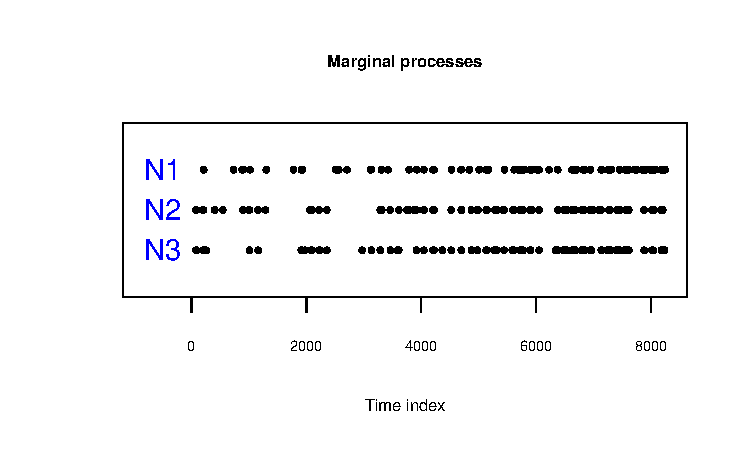
\includegraphics[width=10cm]{figure/Sev1-1} 
\caption{Plot from \code{PlotMargP}: Point processes of the occurrences times of the  EHEs in  Barcelona ($N1$), Huesca ($N2$), and Zaragoza ($N3$).}
\end{figure}
		
The temperature series are highly correlated,  with   Pearson  coefficients  $\rho_{BH}=0.76$,  $\rho_{BZ}=0.73$,  and $\rho_{HZ}=0.94$, but to measure their extremal dependence, a more specific measure, such as the extremal dependence coefficients are used. The functions for the analysis between  $TxZ$ and $TxB$ are shown as an example,  but the pairwise dependence between the three locations is analyzed.

\begin{example}
R> aux<-depchi(TxB,TxZ,indgraph=FALSE,xlegend='topright',
               thresval=c(9000:9975)/10000)
\end{example}
\vspace*{-0.8cm}	
\begin{figure}[h]
	\begin{center}
	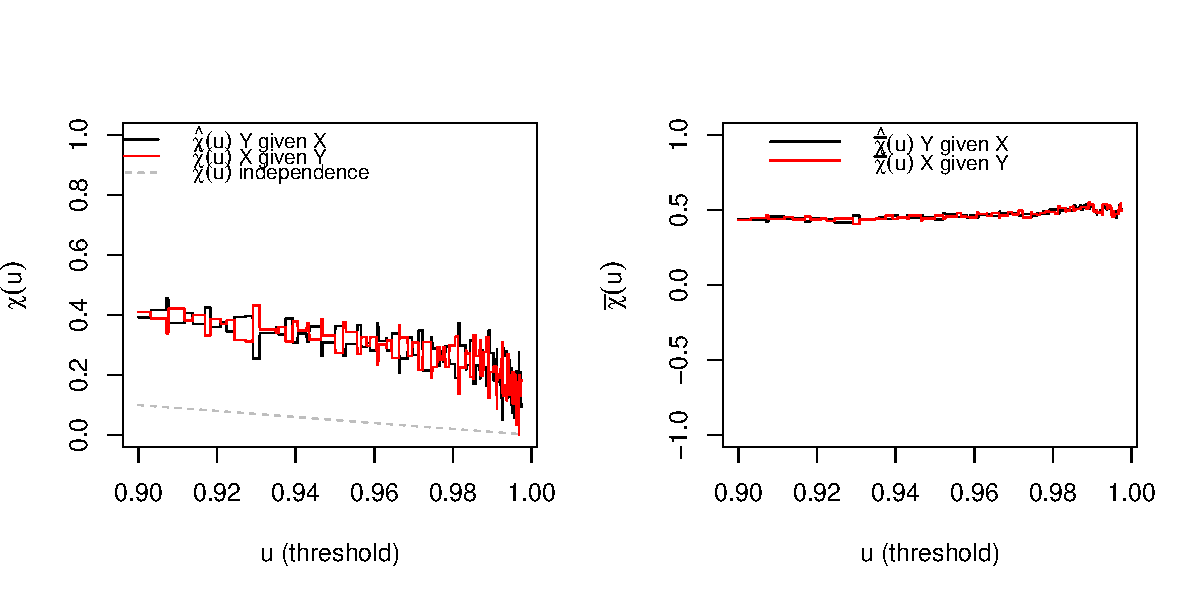
\includegraphics[width=12cm]{figure/Sev2-1} 
	\caption{Plots from \code{depchi} of  $\hat \chi_{x|y}(u)$ and $ \hat{\bar \chi}_{x|y}(u)$  to estimate the extremal dependence coefficients.}
	\end{center}
\end{figure}



The   estimators  $\hat \chi_{B|Z}=\hat \chi_{Z|B}=0$ and  $\hat{\bar \chi}_{B|Z}=\hat{\bar \chi}_{Z|B}=0.5$ suggest an asymptotic independence between   $TxB$ and $TxZ$.  However,  $\hat{\bar \chi}_{Z|B}>0$  suggests dependence  at extreme levels, in particular in the threshold   $\hat  \chi_{Z|B}(0.95) \approx 0.38$.  Similar conclusions are obtained for $TxB$ and $TxH$, while $TxH$ and $TxZ$ are asymptotically dependent, with $\hat \chi_{H|Z}=\hat \chi_{Z|H}=0.5$, $\hat{\bar \chi}_{Z|H}=\hat{\bar \chi}_{H|H}=1$, and   $\hat  \chi_{Z|H}(0.95) \approx 0.7$.

The functions \code{CountingCor}  and \code{BinPer} calculate another extremal dependence  measures,  the correlation coefficient between the number of EHEs in intervals of a given length $ll$, and  the percentage of  concordant intervals,

\begin{example}
R> aux<-CountingCor(posB,posZ, ll=10, T=T, method='kendall')
R> aux

  tau 
  0.3554213  

R> aux<-BinPer(posB,posZ, ll=10, T=T)

  Percentage of concordant intervals:  0.272
\end{example}
with $ll=10$ days,  to measure short-term dependence. All the correlations,  $\varrho_{BZ}^{10}=0.36$,  $\varrho_{BH}^{10}=0.33$, and $\varrho_{ZH}^{10}=0.68$ are  significantly different  from zero.   Similar conclusions are provided by the percentage of  concordant intervals,  $BP_{BZ}^{10}=0.27$,  $BP_{BH}^{10}=0.25$, and $BP_{ZH}^{10}=0.55$.



The dependence given  the empirical intensity of  one process (obtained by  function \code{emplambda.fun} in \pkg{NHPoisson}) can be graphically analyzed using the Dutilleul plot. Figure \ref{FigDutilleul1}  shows the plot  for Zaragoza-Barcelona, resulting  from the following   commands, and  the  plots for  Barcelona-Huesca and Zaragoza-Huesca. 		All the previous results and the plots show that there exists a pairwise  dependence between the  three locations and  that it is stronger between Zaragoza and Huesca. 
 
\begin{example}
R> lambdaEB<-emplambda.fun(posE=posB, t=c(1:T), lint=100, plot=F)$emplambda
R> aux<-DutilleulPlot(posZ, posB, lambdaEB, main="Zaragoza-Barcelona")
\end{example}
	
	
	\begin{figure}[h]
		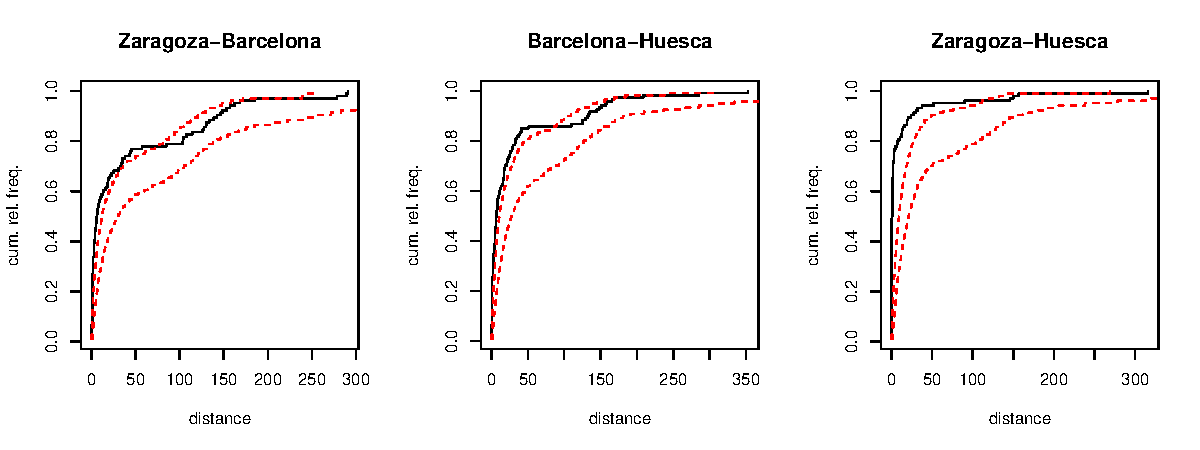
\includegraphics[width=14cm]{figure/Sev5-1} 
		\caption{Dutilleul plot between the pairs of  the EHE processes in the three locations,  given the empirical intensities. \label{FigDutilleul1}}
	\end{figure}
		

		
		
		
\subsection{Testing  independence and analyzing dependence factors}
		
Our next  aim is to   identify the factors which cause the  dependence. To that end, the  independence tests  given the marginal intensities are applied.		
The first step is to model  each  process individually. This has a twofold objective: first, to identify the factors that  influence the occurrence of EHEs  in each series, which may cause the dependence, and  second to  estimate the marginal intensities of the processes. The second step is to check if the  occurrence processes are independent given the fitted intensities. If the  tests  do not reject the null hypothesis, it can be concluded that the dependence between the EHE processes  is explained by the considered covariates since once  its effect is removed, the processes are independent.  The rejection of independence gives evidence that there are other non-identified factors  causing dependence, which have not been included  as predictors in the intensities.
In those cases,  a multivariate model allowing dependence should be used.
		
Step 1. To  model  the occurrence of the EHEs in each series, we  consider a nonhomogeneous Poisson process with an intensity  that is a  function of  a harmonic term  (to model the seasonal behavior) and the  available covariate, which represents the local atmospheric situation  \citep{Abaurrea15}. After the modeling process,  based on a likelihood ratio test, the harmonic term, the covariate,  and the squared covariate  are selected in  Zaragoza. The same terms  are included in Huesca,  and the same plus  interaction between the covariate and the harmonic in Barcelona. These models are fitted using  \code{fitPP.fun} in \pkg{NHPoisson}. The fit of Zaragoza is shown as an example, and the others are carried analogously to obtain $lambdaH$ and $lambdaB$.
		% defined as the moving average of the 15 past days of the series.
		
\begin{example}
R> ss<-sin(2*pi*dayyear/366)
R> cc<-cos(2*pi*dayyear/366)
R> covZ<-cbind(ss,cc, Txm15Z, Txm15Z**2 )
R> dimnames(covZ)<-list(NULL, c("Sin", "Cos", "Txm15", "Txm152"))
R> ModZ<-fitPP.fun(covariates = covZ, posE = posZ,  inddat = auxZ$inddat,
               dplot=F, tit = "Sin+Cos+Txm15+Txm152", 
               start = list(b0 = 1, b1=-1,b2=1, b3=0, b4=0))

  Number of observations  not used in the estimation process:  72
  Total number of time observations:  8262
  Number of events:  104
  Convergence code:  0
  Convergence attained
  Loglikelihood:  -430.087
   
  Estimated coefficients: 
          b0      b1      b2      b3      b4 
     -54.209   0.190  -2.496   2.434  -0.029  
  Full coefficients: 
          b0      b1      b2      b3      b4 
     -54.209   0.190  -2.496   2.434  -0.029 
  attr(,"TypeCoeff")
  [1] "Fixed: No  fixed parameters"

R> lambdaZ<-ModZ@lambdafit
\end{example}
					
The three  fitted  models are satisfactorily validated using  \code{globalval.fun} in \pkg{NHPoisson}.
					
					
Step 2. The independence tests are used to study  the pairwise independence given the fitted intensities. Since it can be assumed that the marginal processes are Poisson,   the three  families of tests POISSON, CLOSE, and CROSS can be  applied.  In the CLOSE family, only  the PaB test is applied since the  processes are nonhomogeneous; in the others, the most powerful test, according to \citet{Cebrian20}, is selected, that is the Normal test and the $K$ test.   Only  the  functions  for the analysis between $TxZ$ and $TxB$ are shown, but all the pairwise comparisons are summarized in Table \ref{Table8}.
					
					
\textbf{POISSON family}. The Normal test is  applied using an interval length  $r=15$ that guarantees the Normal approximation of the statistic.
					
\begin{example}
R> aux<-CondTest(posZ, posB, lambday=lambdaB, r=15)

  WARNING: there are overlapping intervals. The independence hypothesis 
           is not guaranteed.
  The intervals have been shortened to obtain disjoint  intervals.
  The length of the intersection priods are:
  [1] 23 21 28 19 11 12 27 26 20 22 15 27 22 18 18 22 28 16 26 25 17 26 12 26  6
  [26] 8 24 17 28 20 27 20 17 13 17 27 24 23 23 18 27  5 28 10  7 22 27 27 28 23
  [51] 27 26 24 21 19 26 14 14
  The shortest length of the considered intervals is:  3
  The median of the mui values is:  0.5

R> aux$pvN

  Normal p-value 
       0.6859921
\end{example}
								
								
\textbf{CLOSE family}. In the PaB test, the parametric marginal model of the second process,  the  Poisson process  fitted to Barcelona in this case,  has to be specified.  
								
\begin{example}
R> PBZB<-TestIndNH(posZ, posB, nsim = 5000, type = "Poisson", 
         lambdaMarg =cbind(lambdaB), fixed.seed=35)
R> PBZB$pv  

  p-value 
     0.2107578 
\end{example}
											
\textbf{CROSS family}. The $K$ test  is implemented using  an  $r$-grid with values from 1 to 15,  the value selected with the help of the plot of the  estimated  $K(r)$.  Both the \emph{p}-value and  Figure \ref{FigK} suggest the independence  between Z-B given the intensities, since all the values $\hat K(r)$ lie inside the confidence band. On the other hand,  the plot   for Z-H, also shown  in Figure \ref{FigK},  rejects independence for short-term dependence.
\begin{example}
R> auxZB<-NHK(lambdaZ, lambdaB, posC=posZ, posD=posB, r=c(1:15), 
          typePlot='Kfun', cores=2,fixed.seed=36)
R> auxZB$pv

  p-value 
     0.1558442 
\end{example}
\begin{figure}[h]
\begin{center}
		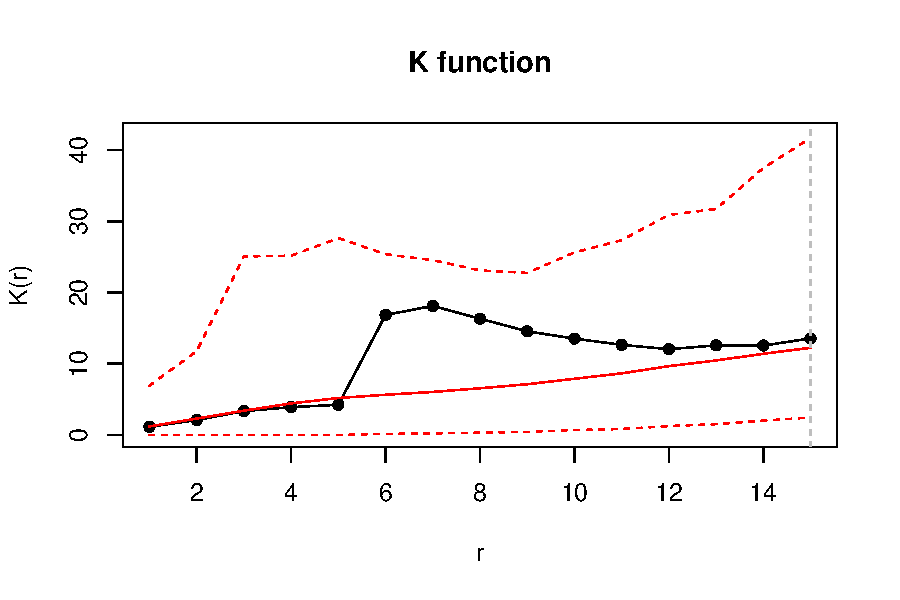
\includegraphics[width=6.5cm]{figure/Sev11-1} 
		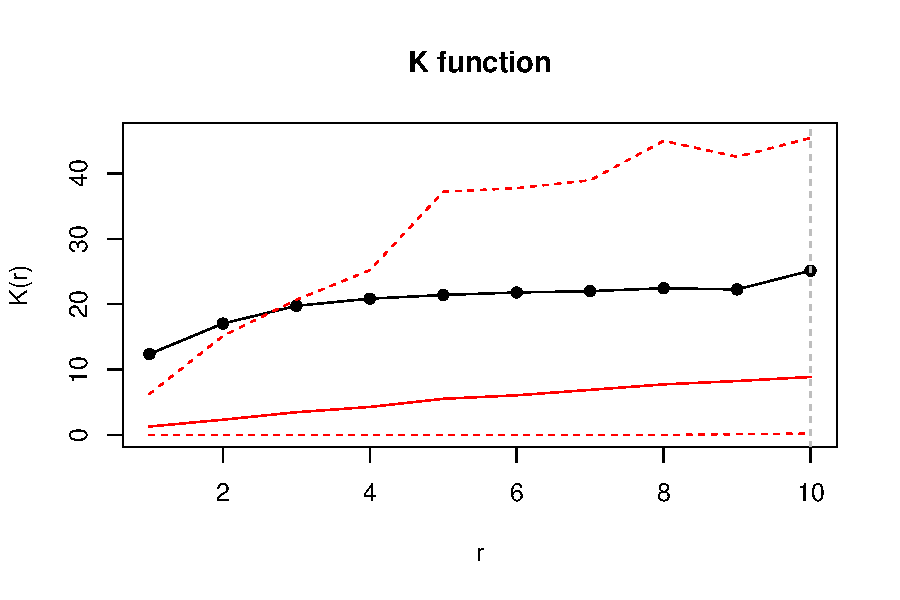
\includegraphics[width=6.5cm]{figure/Sev11-1b} 
\caption{Plot from \code{NHK}: Estimation of the K function and confidence band under independence for Zaragoza-Barcelona (left) and Zaragoza-Huesca (right).\label{FigK}}
\end{center}
\end{figure}
														
														
Table \ref{Table8} summarizes  the three pairwise comparisons.   The three tests lead to the non-rejection of  independence between the occurrences in  B-Z, and to the rejection   between Z-H. On the other hand,   in  pair B-H,  the  $K$  test  rejects the null while all the other tests do not. It is found that  the high value of the  K statistic  is only due to the occurrence of a point  in Huesca in  $t=901$ and  in Barcelona in $t=902$ when the intensity in both locations is  low. In order to analyze the influence of this event, the point in Barcelona is removed, and the  resulting \emph{p}-value, 0.29, does not reject the independence anymore.  
This suggests that the $K$  test is more sensitive than the others to the existence of  an influential point.
Given that  all the tests are built by conditioning  on the occurrences of the first process,   the tests are also applied, changing the order of the locations, and  the same conclusions are obtained. 													
														
\begin{table}[t] \footnotesize	
	\begin{tabular}{cccccccccc}
	\toprule
	 &  \multicolumn{3}{c}{Z-B } &   \multicolumn{3}{c}{B-H}  &  \multicolumn{3}{c}{Z-H} \\ 
	 &  Normal &   PaB  &  $K$  &  Normal &   PaB  &  $K$   &  Normal &   PaB  &  $K$ \\  \midrule		
	  pv  &  .69 &   .21  &  .0.16 & .44  & .25   & .00 (0.29)     & .03 &  .00   & .03 \\ \bottomrule
	\end{tabular}
	\caption{\emph{P}-values of the tests to assess pairwise independence between the occurrence of  EHEs in  Zaragoza, Barcelona, and Huesca.} \label{Table8}
\end{table}
														
These results are graphically confirmed  by the Dutilleul plots given the fitted intensities, where  only the plot  between Zaragoza and Huesca gives evidence of dependence.
														
\begin{example}
R< aux<-DutilleulPlot(posZ, posB, ModB@lambdafit,main="Barcelona-Zaragoza",
       cex.main=0.9)
\end{example}

\begin{figure}[h]
		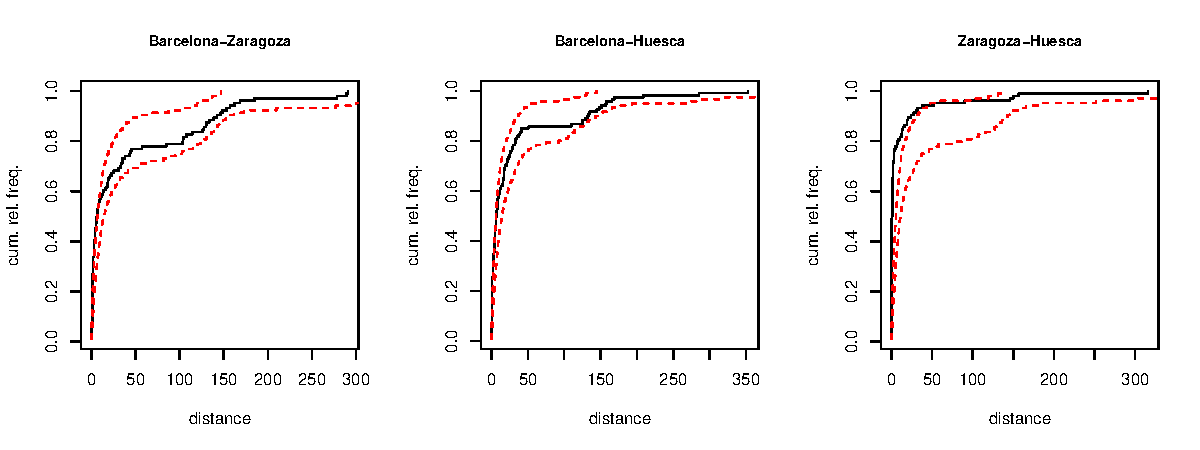
\includegraphics[width=14cm]{figure/Sev12-1} 
		\caption{Dutilleul plot for the pairs of EHE processes  given the fitted intensities. \label{FigDutilleul2}}
\end{figure}
														
The PaB test can also be used  to test  independence between the three processes simultaneously:
														
\begin{example}
R> PBBHZ<-TestIndNH(posB, posH, posZ, nsim = 1000, type = "Poisson",
          lambdaMarg =cbind(lambdaH, lambdaZ), fixed.seed=65, cores=2)  
R< PBBHZ$pv 

  p-value 
     0.002997003 	
\end{example}
																	
Then,  we conclude that, given the fitted  intensities, the occurrence of the EHEs in Zaragoza-Barcelona and Barcelona-Huesca are independent,  while there is  dependence not explained by the covariates in  Zaragoza-Huesca, which are the closest locations. Given these results,   the best model for Barcelona is the previously fitted  model, while the  occurrence processes of Huesca and  Zaragoza should be modeled by a vector of PPs taking into account the dependence between them. A  model  that allows us to include that  dependence  is a CPSP. The occurrences of the three  indicator processes, the process of the events only in Huesca,  only in Zaragoza, and the simultaneous events,  are obtained by the function \code{CPSPPOTevents}. Then,   the CPSP can be estimated by fitting a Poisson process to each of the  three indicator processes using \code{fitPP.fun}; see \citet{Cebrian15} for some examples.
																	
																	
\subsection{Inference  based on computational statistical  methods}
																	
																	
This section   shows two examples of inference based on computational statistical tools using the function \code{IntMPP}. The first example uses the CPSP,  which models the occurrence of EHEs in Huesca and Zaragoza, taking into account the dependence between them.  It is fitted using \pkg{NHPoisson}, and the estimated intensities of the  three indicator processes are  the three last elements of the data.frame \code{TxBHZ}, \code{lambdaOZ}, \code{lambdaOH}, and \code{lambdaZH}.
																	
In the first example,  we calculate  the point estimate and a confidence interval of the time of the first EHE in Zaragoza or Huesca. We need the function \code{firstt}, whose output is the minimum occurrence time  in  a vector of processes.
\begin{example}
R> firstt<-function(posNH){minpos<-min(unlist(posNH))}
R> lambdaiZH<-cbind(lambdaOZ,lambdaOH,lambdaZH)
R> aux<-IntMPP(funMPP.name="DepNHCPSP", 
       funMPP.args=list(lambdaiM=lambdaiZH, d=2, dplot=F), 
       fun.name="firstt", fun.args=NULL, clevel=0.95, cores=2, fixed.seed=125) 

  Lower  bound  of CI:  50.4648
  Point estimator:  116.7493
  Upper bound of CI:  233.4015
\end{example}
																																
This type of inference also allows us to obtain confidence bands for two or more values, for example,  the number of  EHEs in  Huesca and in Zaragoza in a given time interval $I$. To that end, we use the function \code{NumI}, included in the package, whose output is a vector containing the number of points in an interval $I$ in each marginal   process of  a vector of processes. To see the evolution of the number of extremes, we consider  two intervals, the  three first and the three last  years of the period. A clear increase in the number of EHEs is observed in the two locations.
\begin{example}
R> aux<-IntMPP(funMPP.name="DepNHCPSP", 
        funMPP.args=list(lambdaiM=lambdaiZH, d=2, dplot=F),
        fun.name="NumI", fun.args=list(I=c(1,459)),  fixed.seed=125)

  Lower  bound  of CI:  1 1
  Point estimator:  3.058 3.765
  Upper bound of CI:  6 7

R> aux<-IntMPP(funMPP.name="DepNHCPSP", 
         funMPP.args=list(lambdaiM=lambdaiZH, d=2, dplot=FALSE),
         fun.name="NumI", fun.args=list(I=c(7803,8262)), fixed.seed=125)

  Lower  bound  of CI:  9 10
  Point estimator:  15.269 16.952
  Upper bound of CI:  22 24
\end{example}
																	
																	
\subsection{Simulating and characterizing  vectors of processes } 
																	
In this section, some of the  tools  to generate vectors of  processes in \pkg{IndTestPP}  are used to characterize the effect of the dependence in the distribution of the nearest distances between two-point processes. To that end,  two dependent processes with a given dependence structure and two independent processes with the same marginal distribution that the previous ones are generated. The distributions of the  samples of nearest distances are compared using  histograms  and qqplots.  
																	
We generate two dependent Neyman-Scott processes using \code{DepNHNeyScot},  with  mean cluster size equal to 3   and 4, respectively, and  $N(0,3)$ and $N(0,2)$ distributions  for the distances to the center.   The independent processes  with the same marginal distribution are generated using \code{IndNHNeyScot}.  The distribution of the nearest distances is  very different in the two cases, as the qqplot shows.  In the dependent  processes, it is concentrated in  low values, while  in the independent ones the density decreases more smoothly. 
\begin{example}
R> set.seed(123)
R> lambdaParent<-runif(2000)/10

R> aux<-DepNHNeyScot(lambdaParent=lambdaParent, d=2, lambdaNumP=c(3,4), 
        dist="normal", sigmaC=c(3,2),fixed.seed=123, dplot=F)
R> posxd<- aux$posNH$N1
R> posyd<- aux$posNH$N2

R> aux<-IndNHNeyScot(lambdaParent=lambdaParent, d=2, lambdaNumP=c(3,4),
         dist = "normal", sigmaC=c(3,2), fixed.seed=123, dplot=F)
R> posxi<- aux$N1
R> posyi<- aux$N2

R> par(mfrow=c(1,3))
R> distxyd<-nearestdist(posxd , posyd)
R> hist(distxyd , main='Dependent processes', xlab='Nearest dist',
        xlim=c(0,60), ylim=c(0,270),breaks=seq(0,60, by=4) )
R> distxyi<-nearestdist(posxi , posyi)
R> hist(distxyi , main='Independent processes', xlab='Nearest dist',
        xlim=c(0,60), ylim=c(0,270),breaks=seq(0,60, by=4) )
R> qqplot(distxyi, distxyd, xlab='Independent processes', 
          ylab='Dependent processes')
R> lines(distxyd, distxyd, col="red")
\end{example}
\begin{figure}[h]
		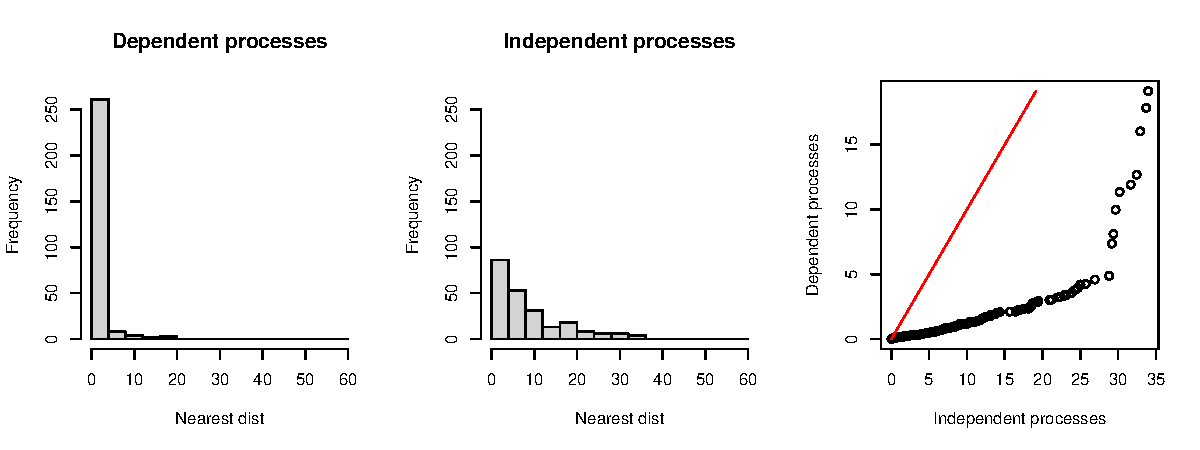
\includegraphics[width=14cm]{figure/Sev14-1} 
		\caption{Histograms of nearest distance in two  dependent and independent MNS processes and qqplot  of the previous nearest distances.}
\end{figure}
															

																	
				
											
\section{Conclusions}


Many modeling problems  related to the occurrence of events require  to analyze the dependence between two or more point processes in time. However, not many tools  to carry out this type of analysis are available.
\pkg{IndTestPP} provides a  useful general framework for applications based on the modeling of a vector of point processes in time since it includes functions   for  processing  data,  estimating the marginal intensities of the processes,   testing independence, identifying factors causing  dependence, and  making an inference. In particular,  the three families of independence tests by \citet{Cebrian20} are implemented. They are  useful in different types of modeling problems  since they cover a wide variety of  processes, homogeneous and nonhomogeneous,  Poisson processes, processes with a  parametric marginal model,  point  processes with  known marginal intensities,  etc.  The package also provides functions to generate  four different types of  vectors of point processes,  Common Poisson Shock processes,  multivariate Neyman-Scott cluster processes,  Poisson processes from queues in a tandem, and  vectors of processes  resulting from a marked Poisson process with discrete marks from  a Markov chain. These generation functions  are used to carry out inference based on computational statistical  methods. The applicability of the package in real modeling problems is shown by analyzing the dependence between the occurrence of extreme temperature events in three Spanish locations, Zaragoza, Barcelona, and Huesca.


\section{Acknowledgements}
	
The authors are members of the research group Modelos Estoc\'asticos (Gobierno de Aragón) and the project MTM2017-83812-P. They   acknowledge  J. Abaurrea and AEMET for the data and their  advice. 
%	The authors thank the  anonymous referees for their valuable comments.
																				


\bibliography{referenciasR}

\address{Ana C. Cebri\'an\\
  University of Zaragoza \\
  Dpto. M\'etodos Estadísticos. Ed. Matemáticas. C Pedro Cerbuna, 12. Zaragoza 50009\\
  Spain \\
  ORCiD: 0000-0002-9052-9674 \\
  \email{acebrian@unizar.es}
}

\address{Jesús Asín\\
	University of Zaragoza \\
	Dpto. M\'etodos Estadísticos. EINA. C María de Luna, 3. Zaragoza 50018         \\
    Spain 
}


